\documentclass{beamer}

\mode<presentation> {
\usetheme{Madrid}
}

\usepackage{graphicx}

\begin{document}

\begin{frame}
\frametitle{Descripcion de un grafico}
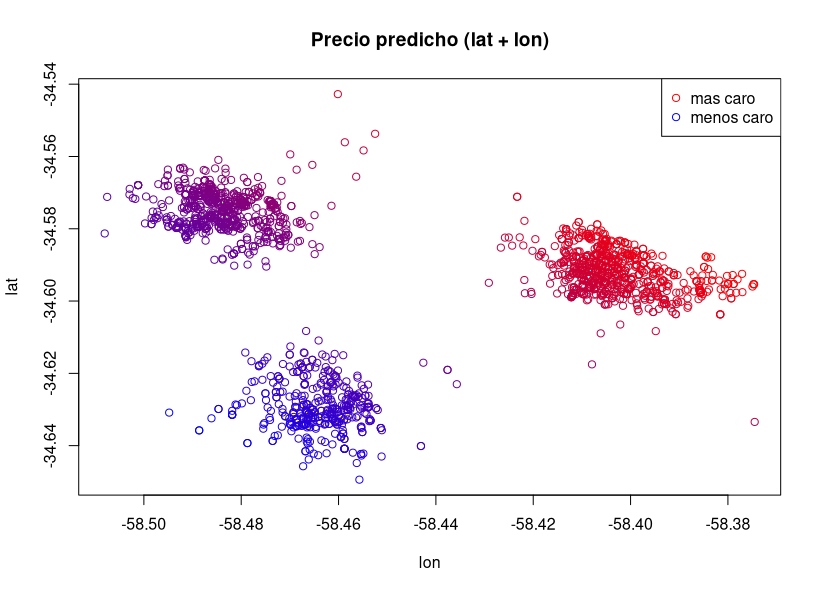
\includegraphics[width=0.95\textwidth]{grafico.png}
\end{frame}

\begin{frame}
\frametitle{Reflexiones}
\begin{itemize}
\item Pros
    \begin{itemize}
    \item Resume cualitativamente al modelo.
    \item Conserva nocion del espacio.
    \item Es lindo (opa).
    \end{itemize}
\item Contras
    \begin{itemize}
    \item Esconde "pendiente" / "momento".
    \item No muestra bondad de ajuste.
    \end{itemize}
\item Mejoras
    \begin{itemize}
    \item Representar magnitudes.
    \item Etiquetar barrios.
    \item Distinguir valores extremos.
    \end{itemize}
\end{itemize}
\end{frame}

\end{document} 